\documentclass[a4paper]{article}

\usepackage{INTERSPEECH2016}

\usepackage{graphicx}
\usepackage{amssymb,amsmath,bm}
\usepackage{textcomp}

\def\vec#1{\ensuremath{\bm{{#1}}}}
\def\mat#1{\vec{#1}}


\sloppy % better line breaks
\ninept

\title{Segmentation of birdsong}

%%%%%%%%%%%%%%%%%%%%%%%%%%%%%%%%%%%%%%%%%%%%%%%%%%%%%%%%%%%%%%%%%%%%%%%%%%
%% If multiple authors, uncomment and edit the lines shown below.       %%
%% Note that each line must be emphasized {\em } by itself.             %%
%% (by Stephen Martucci, author of spconf.sty).                         %%
%%%%%%%%%%%%%%%%%%%%%%%%%%%%%%%%%%%%%%%%%%%%%%%%%%%%%%%%%%%%%%%%%%%%%%%%%%
%\makeatletter
%\def\name#1{\gdef\@name{#1\\}}
%\makeatother
%\name{{\em Firstname1 Lastname1, Firstname2 Lastname2, Firstname3 Lastname3,}\\
%      {\em Firstname4 Lastname4, Firstname5 Lastname5, Firstname6 Lastname6,
%      Firstname7 Lastname7}}
%%%%%%%%%%%%%%% End of required multiple authors changes %%%%%%%%%%%%%%%%%

\makeatletter
\def\name#1{\gdef\@name{#1\\}}
\makeatother \name{{\em Author Name$^1$, Co-author Name$^2$}}

\address{$^1$Author Affiliation \\
  $^2$Co-author Affiliation \\
  {\small \tt author@university.edu, coauthor@company.com}
}

%\twoauthors{Karen Sp\"{a}rck Jones.}{Department of Speech and Hearing \\
%  Brittania University, Ambridge, Voiceland \\
%  {\small \tt Karen@sh.brittania.edu} }
%  {Rose Tyler}{Department of Linguistics \\
%  University of Speechcity, Speechland \\
%  {\small \tt RTyler@ling.speech.edu} }

%
\begin{document}

  \maketitle
  %
  \begin{abstract}
  \end{abstract}
  \noindent{\bf Index Terms}: speech recognition, human-computer interaction, computational paralinguistics



  \section{Introduction}

\section{Entropy-based segmentation of birdsong}
The entropy of spectrograms of bird song recordings can be effectively used for distinguishing between background and bird vocalizations \cite{6625329}. Spectrogram of single bird song is generally sparse i.e. high power components acquire only a small portion of time-frequency bins and the background noise of spectrogram is relatively white. Hence  the entropy of sliding time frequency block over spectrogram is low when block contains a signal and is high when only background is covered. 
\subsection{Entropy Calculation}
The time-frequency block of time length \textbf{\textit{w}} and having F frequency bins ranging from \textbf{\textit{f1}} to  \textbf{\textit{fn}} is slided horizontally from beginning to the end of spectrogram. Entropy is calculated for each time-frequency block. \textbf{\textit{p(n,f)}} is power spectrum at time \textbf{\textit{n}} and frequency  \textbf{\textit{f}}.  The entropy is calculated using following equation:

\hspace{1cm}
  $h_{k}=\sum_{n=kT+1}^{kT+w}\sum_{f=f1}^{fn}z(n,f) \ln z(n,f)$

 \hspace{1cm}
 
Here \textbf{\textit{T}} is time-frequency block shift and \textbf{\textit{z(n,f)}} is normalized power spectrum.


\hspace{1cm}
$z(n,f)=\frac {p(n,f)}
{\sum_{n=kT+1}^{kT+w}\sum_{f=f1}^{fn} p(n,f)}$

\hspace{1cm}

The entropy calculated from block is less susceptible to the bursts of background noise in comparison to the entropy calculated at each time instance. 








\subsection{Thresholding to detect change points}

To detect the change points, thresholding is used. First of all, the entropy is smoothed by using moving average. The local minimums and local maximums are calculated on this smoothed entropy. Then the difference between consecutive local minimums and local maximums is calculated. If this difference is greater than pre-defined threshold, then corresponding local minimum is the change point. Two contiguous change points correspond to the start and end of a bird vocalization. These change points can be tracked back to get the start and end time of the vocalization in sound recording. Smoothing entropy helps in decreasing missed detection rate to some extent.    




\subsection{Experimentation and Performance Analysis}

For experimentation, the labeled recordings of Cassin’s Vireo (\textit{Vireo cassinii}) are used \cite{data}. The total duration of recordings is about 45 minutes. Out of 45 minutes, about 5 minutes of recordings correspond to the phrases of Cassin's Vireo. To calculate spectrogram, frame length of 20 ms and increment of  
5 ms is used. The time-frequency window of 138.8 ms is used along with increment of 15 ms to calculate entropy. 

For performance analysis, three metrics i.e. correct detection rate, missed detection rate and false alarm rate are used. These metrics are calculated using following equations:\newline



$\text{Correct (\%)}=\frac{\text{Correctly classified frames}} {\text{Total frames}} \times 100$\newline


$\text{Missed Detection (\%)}=\frac{\text{Call  frames classified as background}} {\text{Total call activity frames}} \times 100$\newline

$\text{False Alarms (\%)}=\frac{\text{Background  frames classified as calls}} {\text{Total background frames}} \times 100$ \newline


%%  write formullae for calculating correct, missed detection and false alarms

Table 1 shows results generated by applying entropy based segmentation with thresholding on different sound recordings. 

  



\begin{table}[]
	\centering
	\caption{Table showing Correct (\%) Missed Detection(\%) and False alarm (\%) for particular thresholds and moving average windows } 
	\label{Table 1}

	\begin{tabular}{|c|c|c|c|c|c|}
		\hline
		\textbf{File} & \textbf{Span} & \textbf{Threshold} & \textbf{Correct (\%)} & \textbf{False Alarm (\%)} & \textbf{Missed Detection (\%)} \\ \hline
		1.wav         & 9             & 1.2                & 77.7                  & 15.6                      & 60.5                           \\
	\hline	2.wav         & 3             & 1.45               & 73                    & 45                        & 25                             \\
		\hline	3.wav         & 3             & 1.5                & 71                    & 22                        & 54                             \\
		\hline	4.wav         & 9             & 1.15               & 75.1              & 21                  & 51.5                       \\
		\hline	5.wav         & 7             & 1.5                & 76.5                  & 18.5                      & 45                             \\
	\hline		6.wav         & 9             & 1.25               & 82.1              & 15.07                  & 32.2                       \\
		\hline	7.wav         & 7             & 1.25               & 79.6              & 17.8                  & 46.7                       \\
		\hline	8.wav         & 9             & 1.15               & 78.8              & 19.3                  & 35.1                      \\
		\hline	9.wav         & 5             & 1.5                & 86.06              & 13.6                  & 17.9                       \\
	\hline		10.wav        & 9             & 1.6                & 79.6              & 18.3                  & 28.31                       \\
		\hline	11.wav        & 3             & 1.45               & 91.1                  & 32.7                      & 7.53                           \\
		\hline	12.wav        & 7             & 1.4                & 85.1              & 11.3                   & 38.1      \\ \hline               	
	 
	\end{tabular}

\end{table}

\subsection{Whitening Spectrogram using PCA before Entropy Calculation}

To whiten the spectrogram (\textit{PS}), the overall mean is calculated. This mean is subtracted from all values of spectrogram matrix. The covariance matrix of mean subtracted spectrogram is calculated. The Eigen values matrix (\textit{S}) and Eigen vectors matrix (\textit{U}) of this covariance matrix are calculated. The spectrogram matrix is whitened using the following equation:

\hspace{1cm}

$WhitePS=diag(\frac{1}{\sqrt{diag(S)+\epsilon}})*\textit{U'}*\textit{PS}$


\hspace{1cm}

The missed detection rate is decreased if whitened spectrogram is used for entropy calculation. This entropy remains almost constant for background but dips enough to mark the presence of bird vocalizations. Even low energy bird vocalizations can detected using entropy calculated from whitened spectrogram. Following figure depicts the difference between entropy calculated from normal spectrogram and whitened spectrogram:

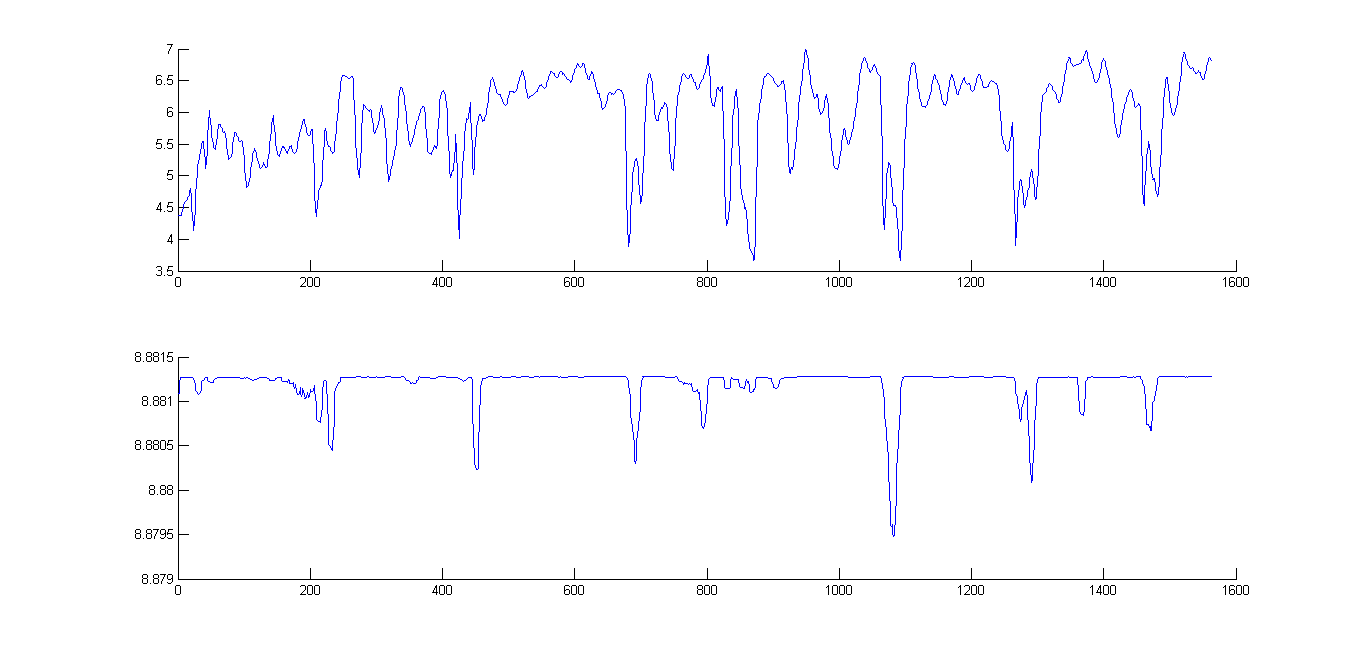
\includegraphics[width=8cm, height=6cm]{entropy}  

  \section{Conclusions}

this is test

  \section{Acknowledgements}
  
    The ISCA Board would like to thank the organizing committees of the past INTERSPEECH conferences for their help and for kindly providing the template files.


  \newpage
  \eightpt
  \bibliographystyle{IEEEtran}

  \bibliography{mybib}

%  \begin{thebibliography}{9}
%    \bibitem[1]{Davis80-COP}
%      S.\ B.\ Davis and P.\ Mermelstein,
%      ``Comparison of parametric representation for monosyllabic word recognition in continuously spoken sentences,''
%      \textit{IEEE Transactions on Acoustics, Speech and Signal Processing}, vol.~28, no.~4, pp.~357--366, 1980.
%    \bibitem[2]{Rabiner89-ATO}
%      L.\ R.\ Rabiner,
%      ``A tutorial on hidden Markov models and selected applications in speech recognition,''
%      \textit{Proceedings of the IEEE}, vol.~77, no.~2, pp.~257-286, 1989.
%    \bibitem[3]{Hastie09-TEO}
%      T.\ Hastie, R.\ Tibshirani, and J.\ Friedman,
%      \textit{The Elements of Statistical Learning -- Data Mining, Inference, and Prediction}.
%      New York: Springer, 2009.
%    \bibitem[4]{YourName16-XXX}
%      F.\ Lastname1, F.\ Lastname2, and F.\ Lastname3,
%      ``Title of your INTERSPEECH 2016 publication,''
%      in \textit{Interspeech 2016 -- 16\textsuperscript{th} Annual Conference of the International Speech Communication Association, September 8–12, San Francisco, California, USA, Proceedings, Proceedings}, 2016, pp.~100--104.
%  \end{thebibliography}

\end{document}
